% Search for all the places that say "PUT SOMETHING HERE".

\documentclass[11pt]{article}
\usepackage{amsmath,textcomp,amssymb,geometry,graphicx,enumerate,bm,hyperref}
\graphicspath{ {images/} }

\title{CS189--FALL 2015 --- Homework 3 Write up}
\author{ZUBO GU, SID 25500921, gu.zubo@berkeley.edu}
\markboth{}{}
\pagestyle{myheadings}
\date{}

\usepackage[procnames]{listings}
\usepackage{color}
\definecolor{keywords}{RGB}{255,0,90}
\definecolor{comments}{RGB}{0,0,113}
\definecolor{red}{RGB}{160,0,0}
\definecolor{green}{RGB}{0,150,0}
 
\lstset{language=Python, 
        basicstyle=\ttfamily\small, 
        keywordstyle=\color{keywords},
        commentstyle=\color{comments},
        stringstyle=\color{red},
        showstringspaces=false,
        identifierstyle=\color{green},
        procnamekeys={def,class}}

\textheight=9in
\textwidth=6.5in
\topmargin=-.75in
\oddsidemargin=0.25in
\evensidemargin=0.25in

\begin{document}
\maketitle

\section*{Problem 1. solution}

\begin{itemize}
\item[1].
See problem1.py file

\item[2].
The residual sum of squares(RSS) is 5.79495380e+12

The predicted value is  -56562.8275451 to 710798.838694. The range is  767361.66624.

It doesn't make sense. All the exact home values are positive in real. Our predicted value has negative value which do not make sense.

\item[3]. 

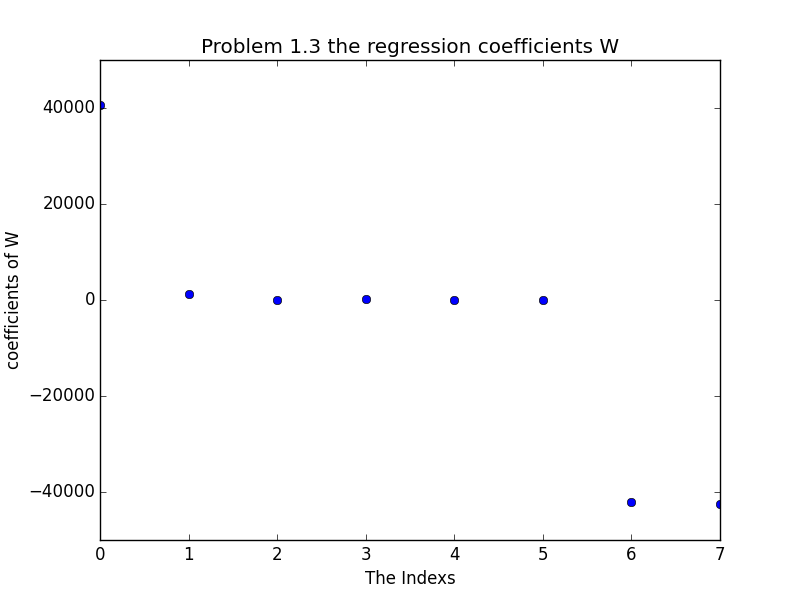
\includegraphics[scale=0.8]{1}

\newpage
\item[4]. 
It is almost normal distribution.

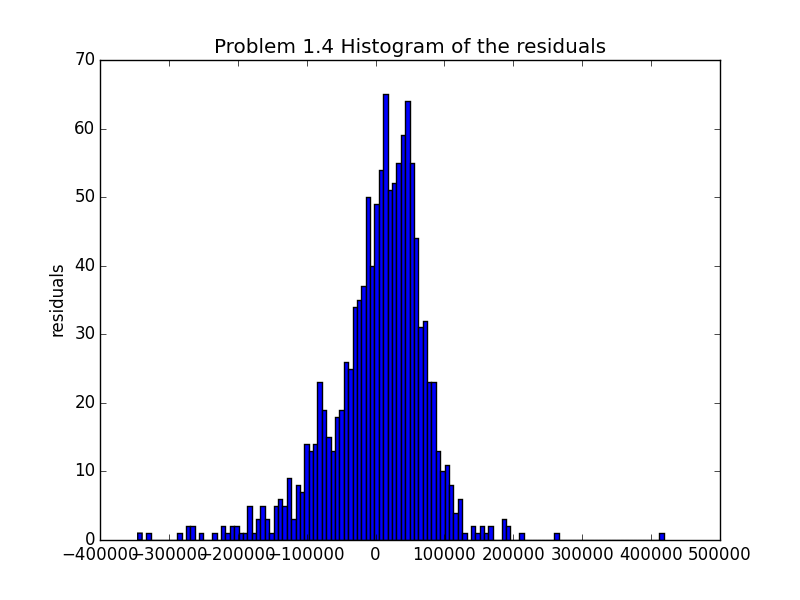
\includegraphics[scale=0.8]{2}

\end{itemize}


\section*{Problem 2. solution}

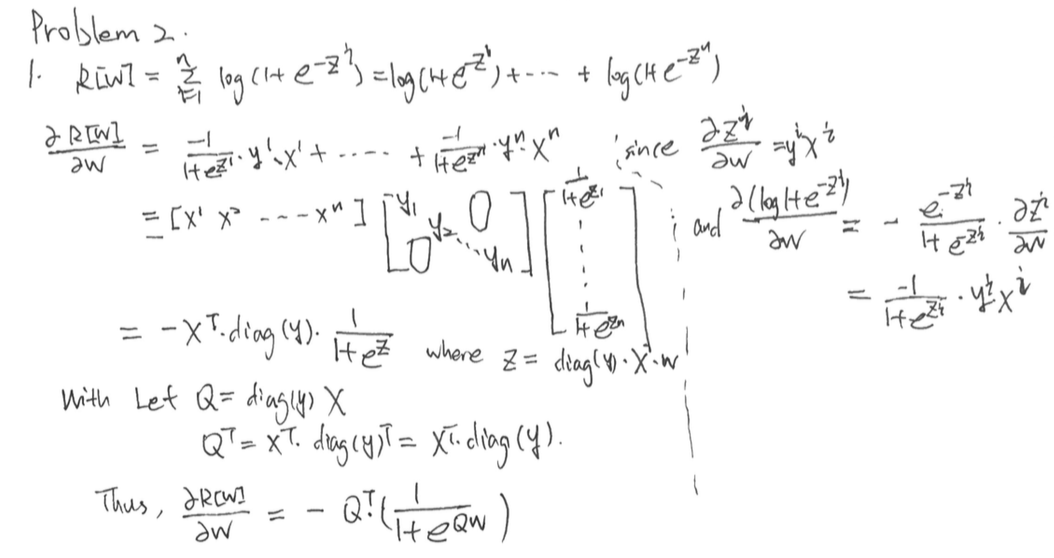
\includegraphics[scale=0.45]{3}

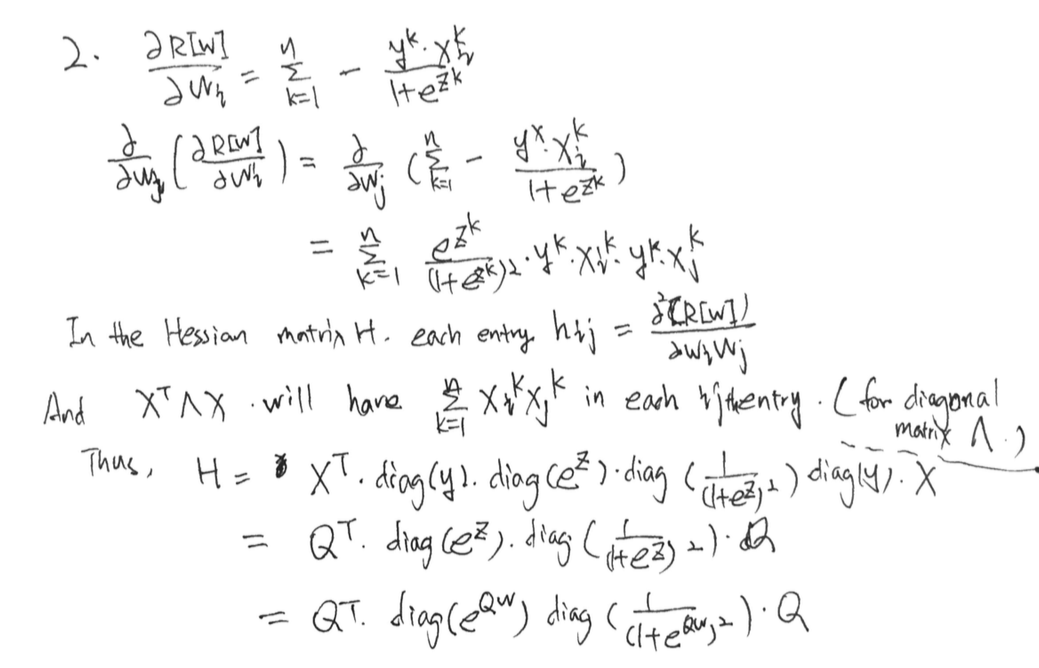
\includegraphics[scale=0.45]{4}
\begin{itemize}
\item[3].

By using code in problem1.py

We can get:

$\mu ^{[0]}$ is [ 0.95257413  0.73105858  0.73105858  0.26894142]

$\omega^{(1)}$ is  [-2.          0.94910188 -0.68363271]

$\mu ^{[1]}$ is [ 0.89693957  0.54082713  0.56598026  0.15000896]

$\omega^{(2)}$ is  [-1.69083609  1.91981257 -0.83738862]


\end{itemize}

\section*{Problem 3. solution}
\begin{itemize}

\item[1].

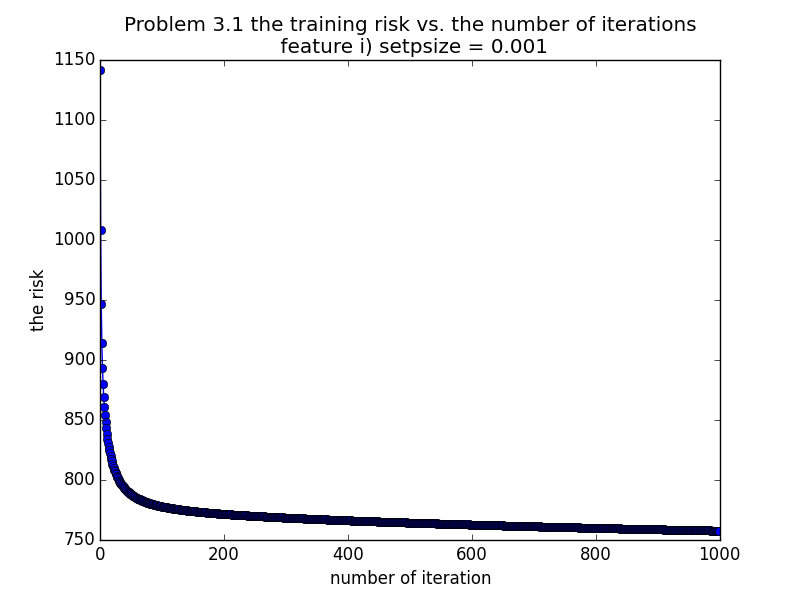
\includegraphics[scale=0.6]{5}

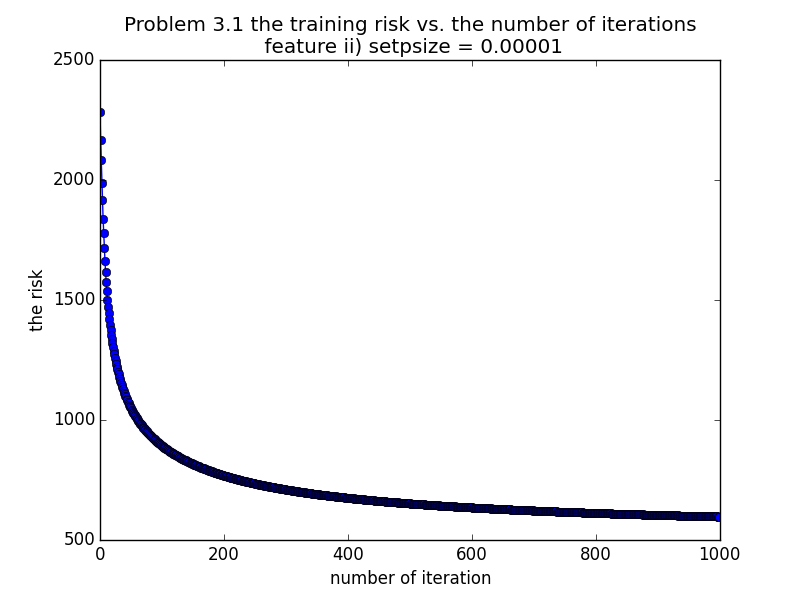
\includegraphics[scale=0.6]{6}

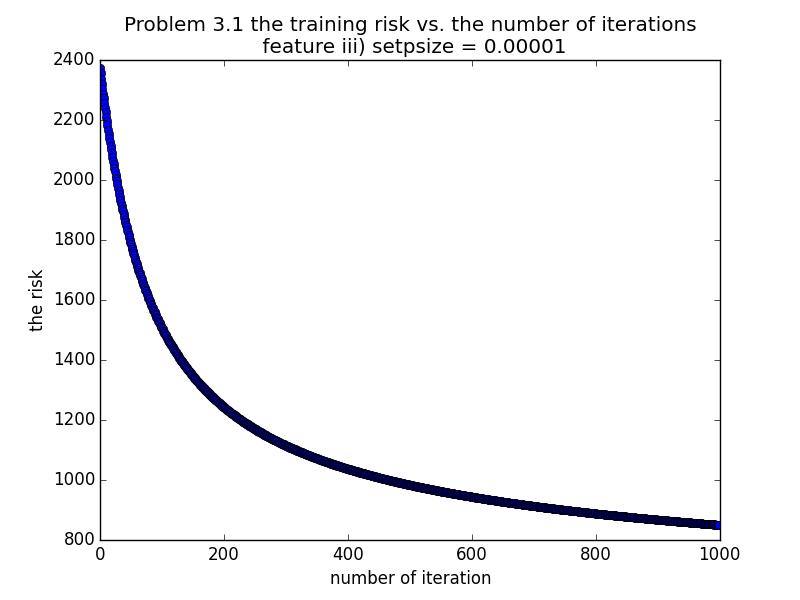
\includegraphics[scale=0.6]{7}

\item[2].

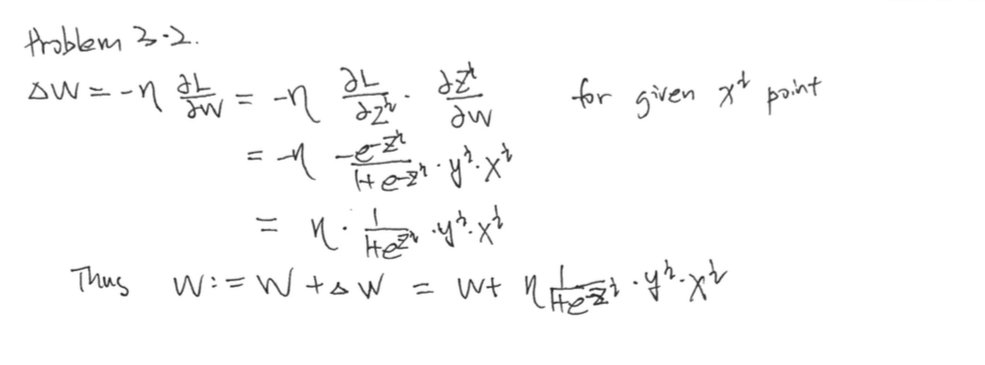
\includegraphics[scale=0.5]{q3_2}

Compare to the plots from (1), with the same iteration, batch gradient descent method is better on reducing the training risk. Also, in the stochastic gradient descent, when we get a bad data point, the training risk even raise.

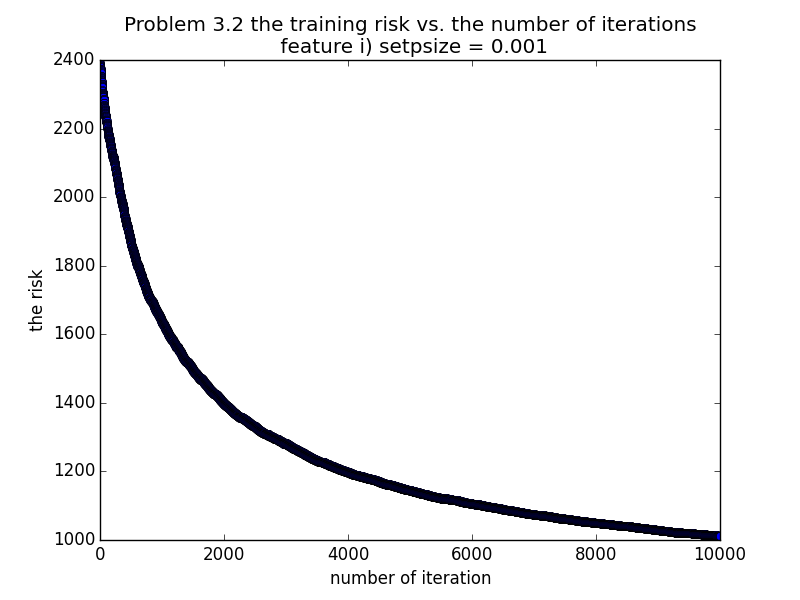
\includegraphics[scale=0.6]{8}

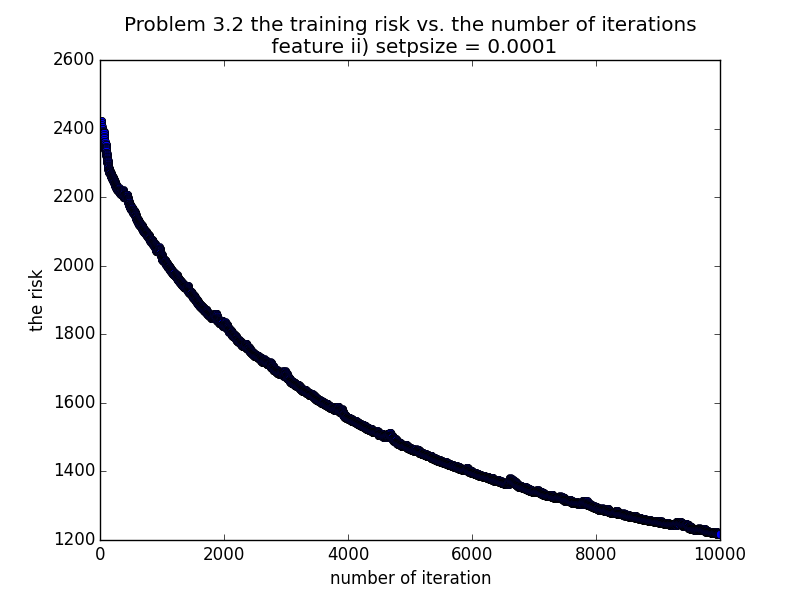
\includegraphics[scale=0.6]{9}

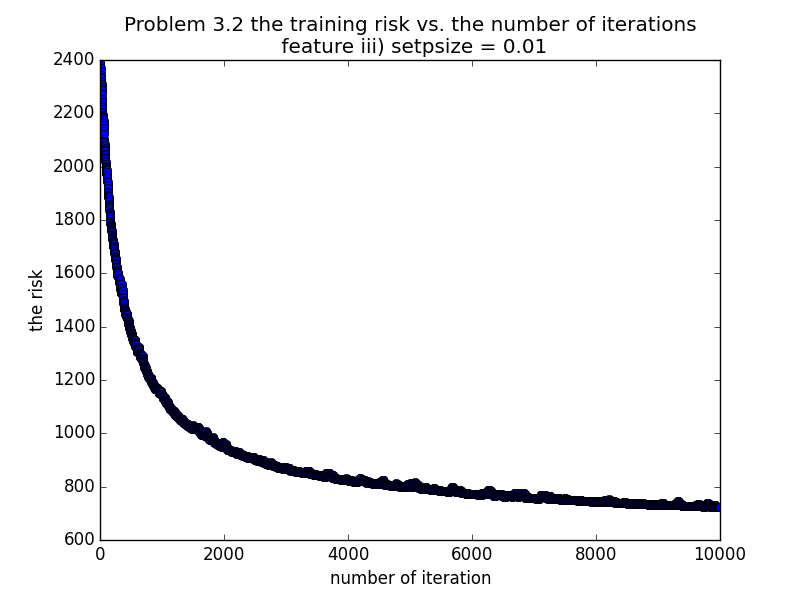
\includegraphics[scale=0.6]{10}


\item[3].

This strategy is much better than having a constant $\eta$ by looking at the graphs.

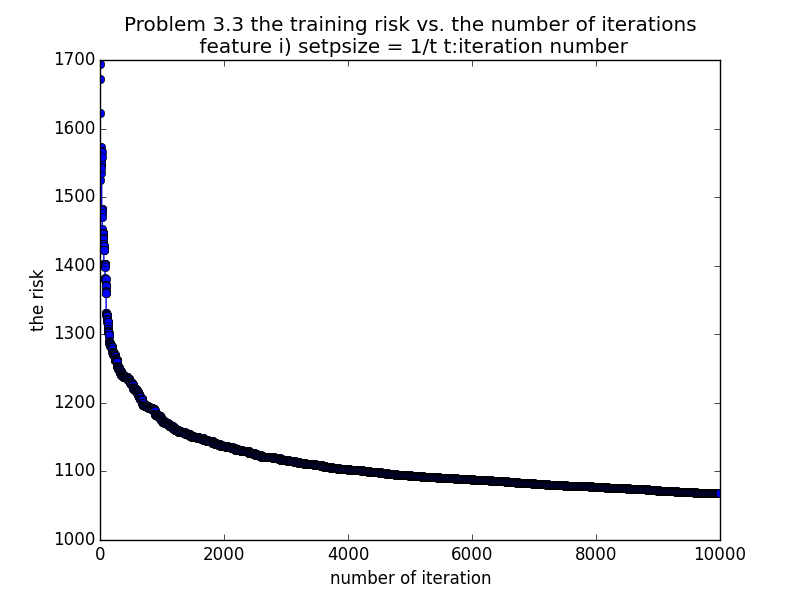
\includegraphics[scale=0.6]{11}

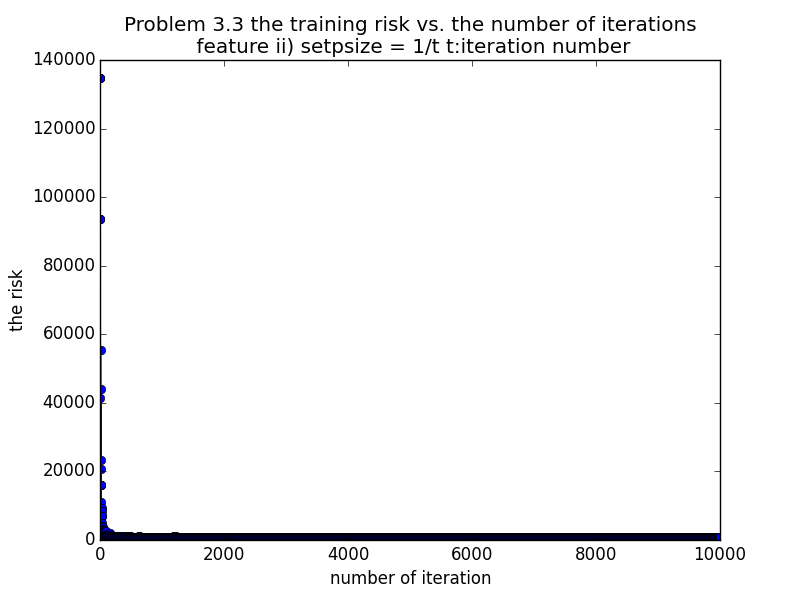
\includegraphics[scale=0.6]{12}

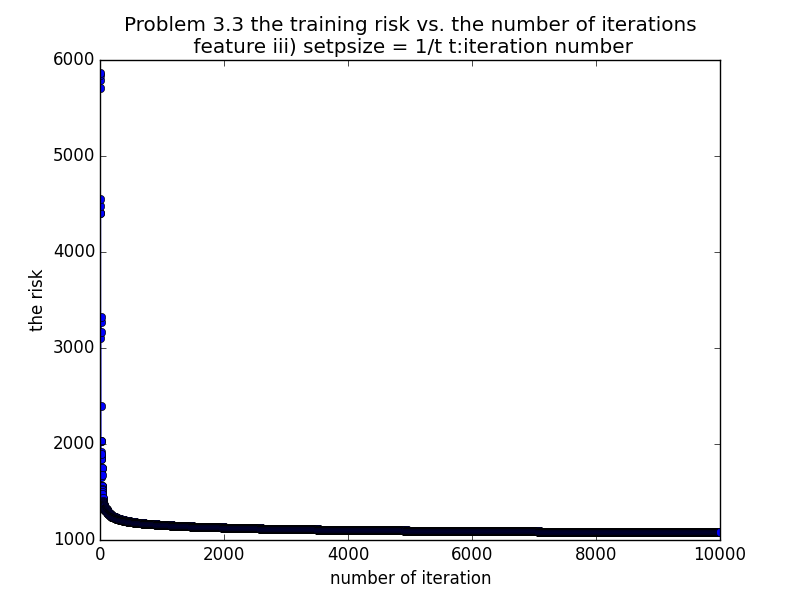
\includegraphics[scale=0.6]{13}

\item[4].

\begin{itemize}
\item[a].

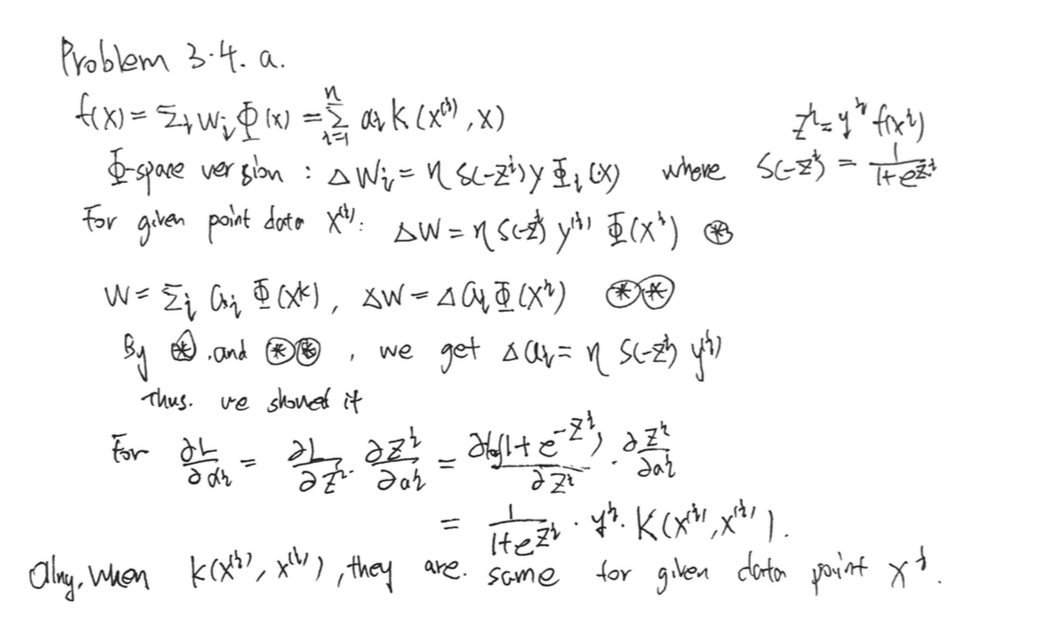
\includegraphics[scale=0.45]{q3_4_a}


\item[b].

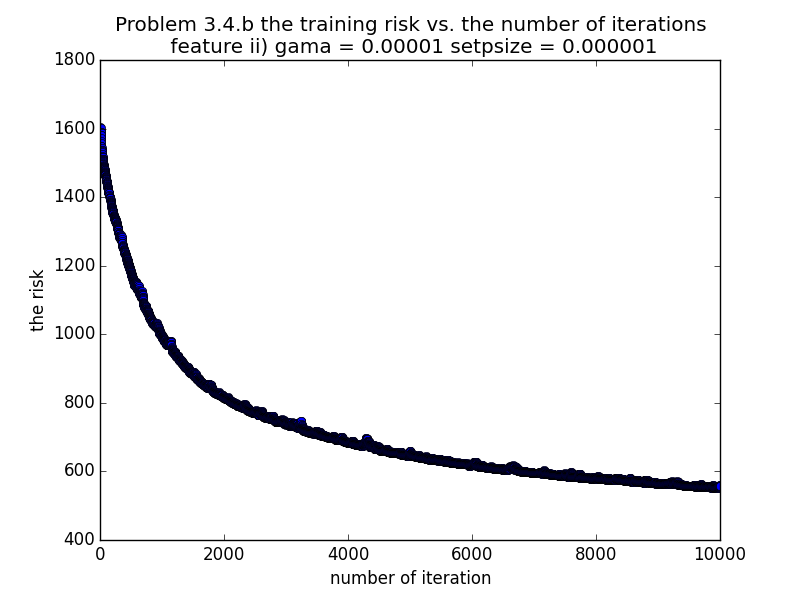
\includegraphics[scale=0.6]{14}

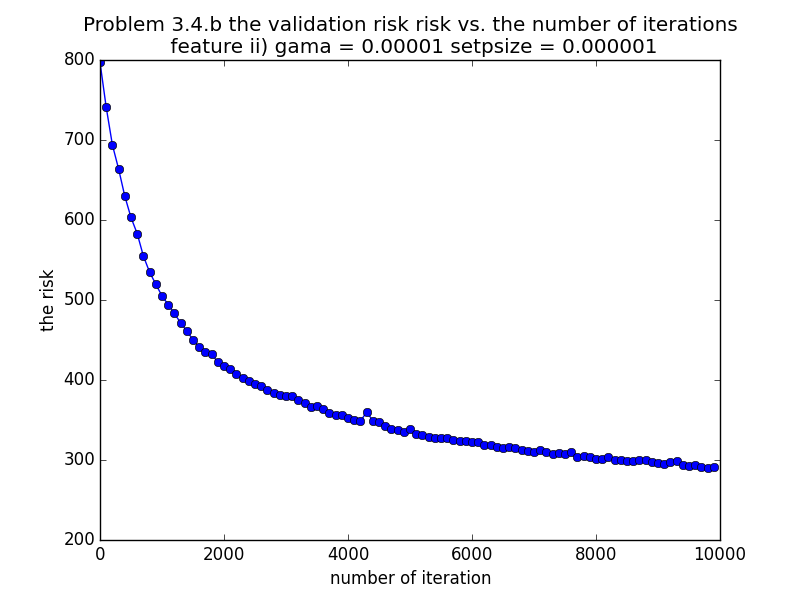
\includegraphics[scale=0.6]{15}

\item[c].

By predict the validation sets of data points and compare to actual validation sets labels as in code, we can see the accuracy for quadratic kernel is even a little bit higher than linear kernel. This means quadratic kernel doesn't overfit the data.

We should decrease $\gamma$ to improve performance.

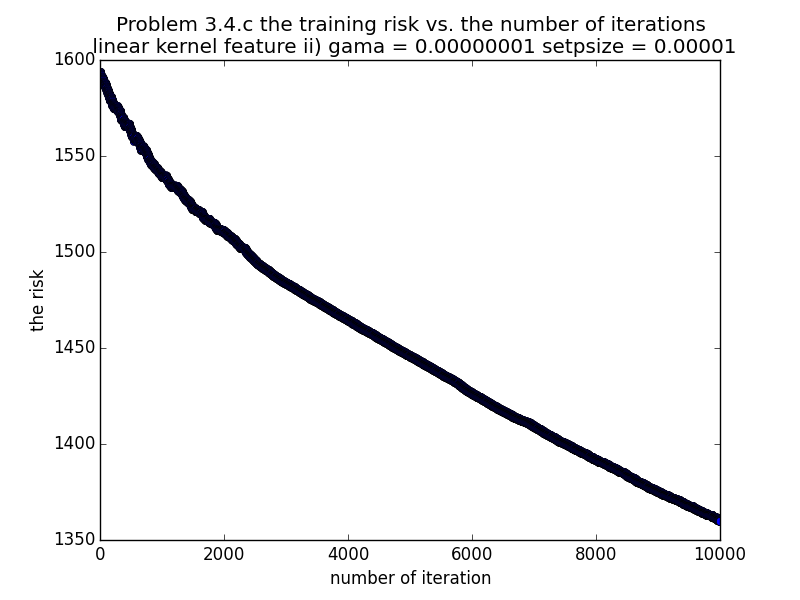
\includegraphics[scale=0.6]{16}

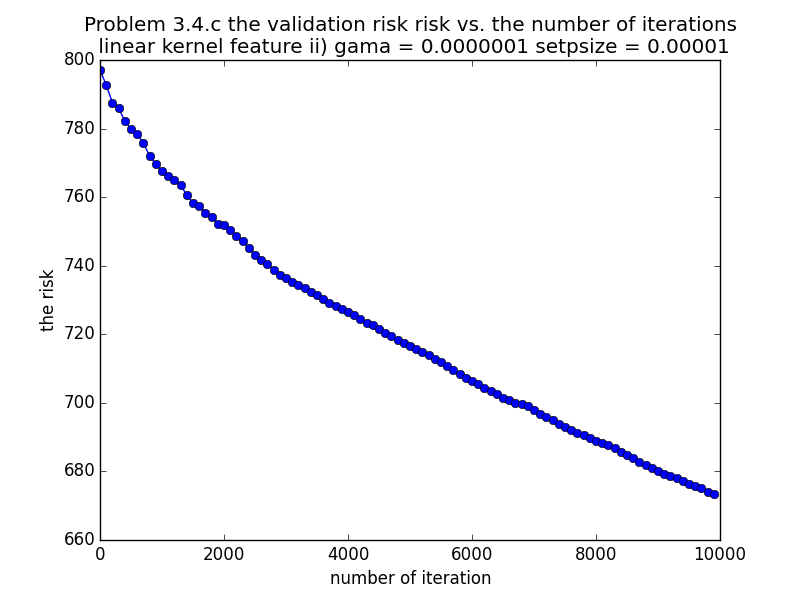
\includegraphics[scale=0.6]{17}

\end{itemize}
\end{itemize}

\section*{Problem 4. solution}
The time-stamp of the received message is very big before the midnight and is very small after the midnight. This adding feature is not linear separable. Thus, the linear SVM didn't work well. In order to improve his results, we need to use a quadratic kernel to improve his model. This adding feature is separable at quadratic kernel.  
\newpage
\begin{lstlisting}
File: problem1.py

import scipy.io as sio
import numpy as np
from numpy.linalg import inv
import matplotlib.pyplot as plt

if __name__ == '__main__':
	#read input
	housingData = sio.loadmat('./data/housing_data.mat')
	# print(housingData)

	#part1 Train the model, get W
	Xvalidate = housingData['Xvalidate']
	Yvalidate = housingData['Yvalidate']
	Xtrain = housingData['Xtrain']
	Ytrain = housingData['Ytrain']
	# print(len(Xvalidate)) #1200
	# print(len(Xvalidate[0])) #8
	# print(len(Yvalidate)) #1200
	# print(len(Xtrain)) #19440
	# print(len(Xtrain[0])) #8

	X = np.insert(Xtrain, 8, 1, axis = 1)
	Xplus = X.T.dot(X)
	Xplus = inv(Xplus)
	W = Xplus.dot(X.T).dot(Ytrain)

	#part2 get the Residual sum of Squares
	Xvalidate1 = np.insert(Xvalidate, 8, 1, axis = 1)
	expect = Xvalidate1.dot(W)
	diff = 0

	sub = expect - Yvalidate
	RSS = 0
	for i in range(len(Yvalidate)):
		RSS += np.square(sub[i])
	print('The RSS is ', RSS)

	print('The predicted value is ', np.min(expect), 'to', np.max(expect))

	print('The range is ', np.max(expect) - np.min(expect))

	print('The exact value is ', np.min(Yvalidate), 'to', np.max(Yvalidate))

	print('The range is ', np.max(Yvalidate) - np.min(Yvalidate))

	#part3 plot W
	W = W[:-1]
	x_label = [0, 1, 2, 3, 4, 5, 6, 7]
	plt.title('Problem 1.3 the regression coefficients W')
	plt.xlabel('The Indexs')
	plt.ylabel('coefficients of W')
	plt.plot(x_label, W, 'bo')
	plt.show()

	#part4 plosy residuals (f(x) - y)
	plt.title('Problem 1.4 Histogram of the residuals')
	plt.ylabel('residuals')
	plt.hist(sub, bins = len(sub)/10)
	plt.show()

\end{lstlisting}

\newpage
\begin{lstlisting}
File:problem2.py

import numpy as np
from numpy.linalg import inv

if __name__ == '__main__':
	X = np.array([[0, 3, 1], [1, 3, 1], [0, 1, 1], [1, 1, 1]])
	y = np.array([1, 1, -1, -1])
	w0 = np.array([-2, 1, 0])
	n = 1

	u0 = 1 / (1 + np.exp(-X.dot(w0.T)))
	print('u0 is', u0)

	Q = np.diag(y).dot(X)
	QW = Q.dot(w0)
	derivateWRTw0 = - Q.T.dot(1 / (1 + np.exp(QW)))
	w1 = w0 - n * derivateWRTw0
	print('w1 is ', w1)

	u1 = 1 / (1 + np.exp(-X.dot(w1.T)))
	print('u1 is', u1)

	QW = Q.dot(w1)
	derivateWRTw1 = - Q.T.dot(1 / (1 + np.exp(QW)))
	w2 = w1 - n * derivateWRTw1
	print('w2 is ', w2)


\end{lstlisting}

\newpage
\begin{lstlisting}
File:problem3.1.py

import scipy.io as sio
import numpy as np
from numpy.linalg import inv
import matplotlib.pyplot as plt
from scipy import stats
from sklearn import preprocessing


def calculateRisk(X, Y, w):
	power = -np.diag(Y).dot(X).dot(w)
	power = power.clip(-99, 99)
	return np.sum(np.log(1 + np.exp(power)))

if __name__ == '__main__':
	#read input
	spamData = sio.loadmat('./data/spam.mat')

	Xtest = spamData['Xtest']
	Xtrain = spamData['Xtrain']
	Ytrain = spamData['Ytrain']
	Ytrain = Ytrain.T[0]

	#standardize each column, so they each have mean 0 and unit variance
	Xstandardize = preprocessing.scale(Xtrain)
	# print(Xstandardize)

	#add bias
	Xtrain = np.insert(Xtrain, 57, 1, axis = 1)

	#transform the feature
	Xtransform = np.log(Xtrain + 0.1)
	# print(Xtransform)

	#Binarize the feature
	binarizer = preprocessing.Binarizer().fit(Xtrain)
	Xbinarize = binarizer.transform(Xtrain)
	# print(Xbinarize)


	#q1
	# #using Xstandardize
	w = np.zeros((57, 1))
	ylabel1 = []
	Q = np.diag(Ytrain).dot(Xstandardize)
	QT = Q.T
	for i in range(1000):
		QW = Q.dot(w)
		QW = QW.clip(-99, 99)
		derivateWRTw = - QT.dot(1 / (1 + np.exp(QW)))
		w = w - 0.001 * derivateWRTw
		risk = calculateRisk(Xstandardize, Ytrain, w)
		ylabel1 += [risk]
		print('The ', i, 'th risk is ', risk)
	x_label1 = [i for i in range(len(ylabel1))]

	plt.title('Problem 3.1 the training risk vs. the number of iterations \n feature i) setpsize = 0.001')
	plt.xlabel('number of iteration')
	plt.ylabel('the risk')
	plt.plot(x_label1, ylabel1, 'bo-')
	plt.show()

	# #using Xtransform
	w = np.zeros((58, 1))
	ylabel2 = []
	Q = np.diag(Ytrain).dot(Xtransform)
	QT = Q.T
	for i in range(1000):
		QW = Q.dot(w)
		QW = QW.clip(-99, 99)
		derivateWRTw = - QT.dot(1 / (1 + np.exp(QW)))
		w = w - 0.00001 * derivateWRTw
		risk = calculateRisk(Xtransform, Ytrain, w)
		ylabel2 += [risk]
		print('The ', i, 'th risk is ', risk)
	x_label2 = [i for i in range(len(ylabel2))]

	plt.title('Problem 3.1 the training risk vs. the number of iterations \n feature ii) setpsize = 0.00001')
	plt.xlabel('number of iteration')
	plt.ylabel('the risk')
	plt.plot(x_label2, ylabel2, 'bo-')
	plt.show()


	# #using Xbinarize
	w = np.zeros((58, 1))
	ylabel3 = []
	Q = np.diag(Ytrain).dot(Xbinarize)
	QT = Q.T
	for i in range(1000):
		QW = Q.dot(w)
		QW = QW.clip(-99, 99)
		derivateWRTw = - QT.dot(1 / (1 + np.exp(QW)))
		w = w - 0.00001 * derivateWRTw
		risk = calculateRisk(Xbinarize, Ytrain, w)
		ylabel3 += [risk]
		print('The ', i, 'th risk is ', risk)
	x_label3 = [i for i in range(len(ylabel3))]

	plt.title('Problem 3.1 the training risk vs. the number of iterations \n feature iii) setpsize = 0.00001')
	plt.xlabel('number of iteration')
	plt.ylabel('the risk')
	plt.plot(x_label3, ylabel3, 'bo-')
	plt.show()

\end{lstlisting}

\newpage
\begin{lstlisting}
File: problem3.2.py

import scipy.io as sio
import numpy as np
from numpy.linalg import inv
import matplotlib.pyplot as plt
from scipy import stats
from sklearn import preprocessing

def calculateRisk(Q, w):
	power = -Q.dot(w)
	power = power.clip(-99, 99)
	return np.sum(np.log(1 + np.exp(power)))

if __name__ == '__main__':
	#read input
	spamData = sio.loadmat('./data/spam.mat')

	Xtest = spamData['Xtest']
	Xtrain = spamData['Xtrain']
	Ytrain = spamData['Ytrain']
	Ytrain = Ytrain.T[0]

	#standardize each column, so they each have mean 0 and unit variance
	Xstandardize = preprocessing.scale(Xtrain)
	# print(Xstandardize)

	#add bias
	Xtrain = np.insert(Xtrain, 57, 1, axis = 1)

	#transform the feature
	Xtransform = np.log(Xtrain + 0.1)
	# print(Xtransform)

	#Binarize the feature
	binarizer = preprocessing.Binarizer().fit(Xtrain)
	Xbinarize = binarizer.transform(Xtrain)
	# print(Xbinarize)


	#q2
	# using Xstandardize
	w = np.zeros((57, 1))
	ylabel1 = []
	Q = np.diag(Ytrain).dot(Xstandardize)
	for i in range(10000):
		index = np.random.randint(0, 3450)	
		xi = np.reshape(Xstandardize[index], (57,1))
		yi = Ytrain[index]
		zi = yi * xi.T.dot(w)
		w = w + 0.001 * yi * xi / (1 + np.exp(zi))
		risk = calculateRisk(Q, w)
		ylabel1 += [risk]
		print('The ', i, 'th risk is ', risk)
	x_label1 = [i for i in range(len(ylabel1))]
	plt.title('Problem 3.2 the training risk vs. the number of iterations \n feature i) setpsize = 0.001')
	plt.xlabel('number of iteration')
	plt.ylabel('the risk')
	plt.plot(x_label1, ylabel1, 'bo-')
	plt.show()

	# #using Xtransform
	w = np.zeros((58, 1))
	ylabel2 = []
	Q = np.diag(Ytrain).dot(Xtransform)
	for i in range(10000):
		index = np.random.randint(0, 3450)	
		xi = np.reshape(Xtransform[index], (58,1))
		yi = Ytrain[index]
		zi = yi * xi.T.dot(w)
		w = w + 0.0001 * yi * xi / (1 + np.exp(zi))
		risk = calculateRisk(Q, w)
		ylabel2 += [risk]
		print('The ', i, 'th risk is ', risk)
	x_label2 = [i for i in range(len(ylabel2))]
	plt.title('Problem 3.2 the training risk vs. the number of iterations \n feature ii) setpsize = 0.0001')
	plt.xlabel('number of iteration')
	plt.ylabel('the risk')
	plt.plot(x_label2, ylabel2, 'bo-')
	plt.show()


	# # #using Xbinarize
	w = np.zeros((58, 1))
	ylabel3 = []
	Q = np.diag(Ytrain).dot(Xbinarize)
	for i in range(10000):
		index = np.random.randint(0, 3450)	
		xi = np.reshape(Xbinarize[index], (58,1))
		yi = Ytrain[index]
		zi = yi * xi.T.dot(w)
		w = w + 0.01 * yi * xi / (1 + np.exp(zi))
		risk = calculateRisk(Q, w)
		ylabel3 += [risk]
		print('The ', i, 'th risk is ', risk)
	x_label3 = [i for i in range(len(ylabel3))]
	plt.title('Problem 3.2 the training risk vs. the number of iterations \n feature iii) setpsize = 0.01')
	plt.xlabel('number of iteration')
	plt.ylabel('the risk')
	plt.plot(x_label3, ylabel3, 'bo-')
	plt.show()

\end{lstlisting}

\newpage
\begin{lstlisting}
File: problem3.3.py

import scipy.io as sio
import numpy as np
from numpy.linalg import inv
import matplotlib.pyplot as plt
from scipy import stats
from sklearn import preprocessing

def calculateRisk(Q, w):
	power = -Q.dot(w)
	power = power.clip(-99, 99)
	return np.sum(np.log(1 + np.exp(power)))

if __name__ == '__main__':
	#read input
	spamData = sio.loadmat('./data/spam.mat')

	Xtest = spamData['Xtest']
	Xtrain = spamData['Xtrain']
	Ytrain = spamData['Ytrain']
	Ytrain = Ytrain.T[0]

	#standardize each column, so they each have mean 0 and unit variance
	Xstandardize = preprocessing.scale(Xtrain)
	# print(Xstandardize)

	#add bias
	Xtrain = np.insert(Xtrain, 57, 1, axis = 1)

	#transform the feature
	Xtransform = np.log(Xtrain + 0.1)
	# print(Xtransform)

	#Binarize the feature
	binarizer = preprocessing.Binarizer().fit(Xtrain)
	Xbinarize = binarizer.transform(Xtrain)
	# print(Xbinarize)

	#q2
	# using Xstandardize
	w = np.zeros((57, 1))
	ylabel1 = []
	Q = np.diag(Ytrain).dot(Xstandardize)
	for i in range(10000):
		index = np.random.randint(0, 3450)	
		xi = np.reshape(Xstandardize[index], (57,1))
		yi = Ytrain[index]
		zi = yi * xi.T.dot(w)
		w = w + yi * xi / (1 + np.exp(zi)) / (i + 1)
		risk = calculateRisk(Q, w)
		ylabel1 += [risk]
		print('The ', i, 'th risk is ', risk)
	x_label1 = [i for i in range(len(ylabel1))]

	plt.title('Problem 3.3 the training risk vs. the number of iterations \n feature i) setpsize = 1/t t:iteration number')
	plt.xlabel('number of iteration')
	plt.ylabel('the risk')
	plt.plot(x_label1, ylabel1, 'bo-')
	plt.show()

	#using Xtransform
	w = np.zeros((58, 1))
	ylabel2 = []
	Q = np.diag(Ytrain).dot(Xtransform)
	for i in range(10000):
		index = np.random.randint(0, 3450)	
		xi = np.reshape(Xtransform[index], (58,1))
		yi = Ytrain[index]
		zi = yi * xi.T.dot(w)
		w = w + yi * xi / (1 + np.exp(zi)) / (i + 1)
		risk = calculateRisk(Q, w)
		ylabel2 += [risk]
		print('The ', i, 'th risk is ', risk)
	x_label2 = [i for i in range(len(ylabel2))]
	plt.title('Problem 3.3 the training risk vs. the number of iterations \n feature ii) setpsize = 1/t t:iteration number')
	plt.xlabel('number of iteration')
	plt.ylabel('the risk')
	plt.plot(x_label2, ylabel2, 'bo-')
	plt.show()


	# #using Xbinarize
	w = np.zeros((58, 1))
	ylabel3 = []
	Q = np.diag(Ytrain).dot(Xbinarize)
	for i in range(10000):
		index = np.random.randint(0, 3450)	
		xi = np.reshape(Xbinarize[index], (58,1))
		yi = Ytrain[index]
		zi = yi * xi.T.dot(w)
		w = w + yi * xi / (1 + np.exp(zi)) / (i + 1)
		risk = calculateRisk(Q, w)
		ylabel3 += [risk]
		print('The ', i, 'th risk is ', risk)
	x_label3 = [i for i in range(len(ylabel3))]
	plt.title('Problem 3.3 the training risk vs. the number of iterations \n feature iii) setpsize = 1/t t:iteration number')
	plt.xlabel('number of iteration')
	plt.ylabel('the risk')
	plt.plot(x_label3, ylabel3, 'bo-')
	plt.show()



\end{lstlisting}


\newpage
\begin{lstlisting}
File: problem.3.4.b.py

import scipy.io as sio
import numpy as np
from numpy.linalg import inv
import matplotlib.pyplot as plt
from scipy import stats
from sklearn import preprocessing
import random

def calculateRisk(Y, alpha, sum1):
	fx = sum1.dot(alpha)
	power = - np.diag(Y).dot(fx)
	power = power.clip(-99, 99)
	return np.sum(np.log(1 + np.exp(power)))

if __name__ == '__main__':
	#read input
	spamData = sio.loadmat('./data/spam.mat')

	Xtest = spamData['Xtest']
	Xtrain = spamData['Xtrain']
	Ytrain = spamData['Ytrain']
	Ytrain = Ytrain.T[0]

	#standardize each column, so they each have mean 0 and unit variance
	#add bias
	Xtrain = np.insert(Xtrain, 57, 1, axis = 1)

	#transform the feature
	Xtransform = np.log(Xtrain + 0.1)
	# print(Xtransform)

	#partition samples
	samples_indexs = [i for i in range(3450)]
	random.shuffle(samples_indexs)
	validation_sets_index = samples_indexs[:1150]
	validation_sets = []
	validation_sets_labels = []
	samples_sets = []
	samples_sets_labels = []
	for index in validation_sets_index:
		validation_sets += [Xtransform[index]]
		validation_sets_labels += [Ytrain[index]]
	samples_indexs = samples_indexs[1150:3450]
	for index in samples_indexs:
		samples_sets += [Xtransform[index]]
		samples_sets_labels += [Ytrain[index]]

	validation_sets = np.array(validation_sets)
	validation_sets_labels = np.array(validation_sets_labels)
	samples_sets = np.array(samples_sets)
	samples_sets_labels = np.array(samples_sets_labels)		

	#part b
	# using Xtransform
	alpha = np.zeros((2300, 1))
	gama = 0.00001
	ylabel1 = []
	ylabel2 = []
	sum1 = np.square(samples_sets.dot(samples_sets.T) + 1) # for trianng set
	sum2 = np.square(validation_sets.dot(samples_sets.T) + 1) # for validation set
	for i in range(10000):
		if i % 100 == 0:
			validationRisk = calculateRisk(validation_sets_labels, alpha, sum2)
			ylabel2 += [validationRisk]
			print('The ', i, 'th risk is ', validationRisk)
		index = np.random.randint(0, 2300)	
		xi = np.reshape(samples_sets[index], (58,1))
		yi = samples_sets_labels[index]
		zi = yi * alpha.T.dot(np.square(samples_sets.dot(xi) + 1))
		zi = zi.clip(-99, 99)
		alpha[index] = alpha[index] + 0.000001 * yi / (1 + np.exp(zi))
		alpha = (1 - gama) * alpha
		risk = calculateRisk(samples_sets_labels, alpha, sum1)
		ylabel1 += [risk]
		# print('The ', i, 'th risk is ', risk)
	x_label1 = [i for i in range(len(ylabel1))]
	x_label2 = [i * 100 for i in range(len(ylabel2))]

	pred = []
	for i in range(1150):
		xi = np.reshape(validation_sets[i], (58,1))
		fx = alpha.T.dot(np.square(samples_sets.dot(xi) + 1))
		probbe1 = 1 / (1 + np.exp(-fx))
		if probbe1 > 0.5:
			pred += [1]
		else:
			pred += [-1]

	same = [i for i in range(1150) if pred[i] == validation_sets_labels[i]]

	print('the accuracy is', len(same)/1150)

	plt.title('Problem 3.4.b the training risk vs. the number of iterations \n feature ii) gama = 0.00001 setpsize = 0.000001')
	plt.xlabel('number of iteration')
	plt.ylabel('the risk')
	plt.plot(x_label1, ylabel1, 'bo-')
	plt.show()

	plt.title('Problem 3.4.b the validation risk risk vs. the number of iterations \n feature ii) gama = 0.00001 setpsize = 0.000001')
	plt.xlabel('number of iteration')
	plt.ylabel('the risk')
	plt.plot(x_label2, ylabel2, 'bo-')
	plt.show()



\end{lstlisting}



\newpage
\begin{lstlisting}
File: problem3.4.c.py

import scipy.io as sio
import numpy as np
from numpy.linalg import inv
import matplotlib.pyplot as plt
from scipy import stats
from sklearn import preprocessing
import random

def calculateRisk(Y, alpha, sum1):
	fx = sum1.dot(alpha)
	power = - np.diag(Y).dot(fx)
	power = power.clip(-99, 99)
	return np.sum(np.log(1 + np.exp(power)))

if __name__ == '__main__':
	#read input
	spamData = sio.loadmat('./data/spam.mat')

	Xtest = spamData['Xtest']
	Xtrain = spamData['Xtrain']
	Ytrain = spamData['Ytrain']
	Ytrain = Ytrain.T[0]

	#standardize each column, so they each have mean 0 and unit variance
	#add bias
	Xtrain = np.insert(Xtrain, 57, 1, axis = 1)

	#transform the feature
	Xtransform = np.log(Xtrain + 0.1)
	# print(Xtransform)

	#partition samples
	samples_indexs = [i for i in range(3450)]
	random.shuffle(samples_indexs)
	validation_sets_index = samples_indexs[:1150]
	validation_sets = []
	validation_sets_labels = []
	samples_sets = []
	samples_sets_labels = []
	for index in validation_sets_index:
		validation_sets += [Xtransform[index]]
		validation_sets_labels += [Ytrain[index]]
	samples_indexs = samples_indexs[1150:3450]
	for index in samples_indexs:
		samples_sets += [Xtransform[index]]
		samples_sets_labels += [Ytrain[index]]

	validation_sets = np.array(validation_sets)
	validation_sets_labels = np.array(validation_sets_labels)
	samples_sets = np.array(samples_sets)
	samples_sets_labels = np.array(samples_sets_labels)		

	#part c
	alpha = np.zeros((2300, 1))
	gama = 0.00000001
	ylabel1 = []
	ylabel2 = []
	sum1 = samples_sets.dot(samples_sets.T) + 1 # for trianng set
	sum2 = validation_sets.dot(samples_sets.T) + 1 # for validation set
	for i in range(10000):
		if i % 100 == 0:
			validationRisk = calculateRisk(validation_sets_labels, alpha, sum2)
			ylabel2 += [validationRisk]
			print('The ', i, 'th risk is ', validationRisk)
		index = np.random.randint(0, 2300)	
		xi = np.reshape(samples_sets[index], (58,1))
		yi = samples_sets_labels[index]
		zi = yi * alpha.T.dot(samples_sets.dot(xi) + 1)
		zi = zi.clip(-99, 99)
		alpha[index] = alpha[index] + 0.00001 * yi / (1 + np.exp(zi))
		alpha = (1 - gama) * alpha
		risk = calculateRisk(samples_sets_labels, alpha, sum1)
		ylabel1 += [risk]
		# print('The ', i, 'th risk is ', risk)
	x_label1 = [i for i in range(len(ylabel1))]
	x_label2 = [i * 100 for i in range(len(ylabel2))]


	pred = []
	for i in range(1150):
		xi = np.reshape(validation_sets[i], (58,1))
		fx = alpha.T.dot(np.square(samples_sets.dot(xi) + 1))
		probbe1 = 1 / (1 + np.exp(-fx))
		if probbe1 > 0.5:
			pred += [1]
		else:
			pred += [-1]

	same = [i for i in range(1150) if pred[i] == validation_sets_labels[i]]

	print('the accuracy is', len(same)/1150)

	plt.title('Problem 3.4.c the training risk vs. the number of iterations \n linear kernel feature ii) gama = 0.00000001 setpsize = 0.00001')
	plt.xlabel('number of iteration')
	plt.ylabel('the risk')
	plt.plot(x_label1, ylabel1, 'bo-')
	plt.show()

	plt.title('Problem 3.4.c the validation risk risk vs. the number of iterations \n linear kernel feature ii) gama = 0.0000001 setpsize = 0.00001')
	plt.xlabel('number of iteration')
	plt.ylabel('the risk')
	plt.plot(x_label2, ylabel2, 'bo-')

\end{lstlisting}




\end{document}